\section{Leak-Free Results: What Helps}
\label{sec:leakfree}

\subsection{The Benchmark at Full Labels}
Table~\ref{tab:leakfree}, Fig.~\ref{fig:benchmark} and Fig.~\ref{fig:perclass} give the benchmark, all scored with one evaluator on cached predictions.

\begin{table}[!t]
\centering
\caption{Leak-free benchmark, full labels: test \mfifty/\mcoco, COCO-style evaluator; mean of two seeds where marked (2), per-seed values in Table~\ref{tab:newruns}. The A0 seeds are the two T4 runs paired with RF-DETR-FP; an A100 rerun of A0 seed 1 scored 54.8/32.2 and 41.0/16.9. Cross-architecture rows have no paired interval, so treat them as point estimates. \hlnote{} Shaded: proposed method.}
\label{tab:leakfree}
\footnotesize
\setlength{\tabcolsep}{3pt}
\begin{tabularx}{\linewidth}{@{}X cc cc@{}}
\toprule
& \multicolumn{2}{c}{WTBD-group} & \multicolumn{2}{c}{WTBlade-group} \\
& \multicolumn{2}{c}{\scriptsize 161 img, 58 scenes} & \multicolumn{2}{c}{\scriptsize 332 frames, 177 scenes} \\
\cmidrule(lr){2-3}\cmidrule(l){4-5}
Model & 50 & 50:95 & 50 & 50:95 \\
\midrule
YOLO12-L & 40.0 & 18.5 & 32.2 & 13.3 \\
BladeYOLO-v2 without DINOv3 & 31.8 & 15.2 & -- & -- \\
BladeYOLO-v2 (ViT-S / ViT-B) & \second{56.1} & 24.4 & \best{41.8} & \best{18.0} \\
RF-DETR-M, A0 (2) & 54.3 & 32.2 & 40.0 & 16.6 \\
\quad + copy-paste, A1 (2) & 55.0 & 31.7 & 40.6 & 16.9 \\
\quad + copy-paste + in-domain SSL, A2 & 49.6 & 27.4 & 40.1 & 16.1 \\
\quad + copy-paste + multi-dataset, A3 & 55.3 & \second{33.2} & \second{41.7} & 16.6 \\
\ours RF-DETR-FP (ours) (2) & \best{58.9} & \best{34.4} & 41.0 & \second{17.3} \\
\bottomrule
\end{tabularx}
\end{table}

\begin{figure*}[!t]
\centering
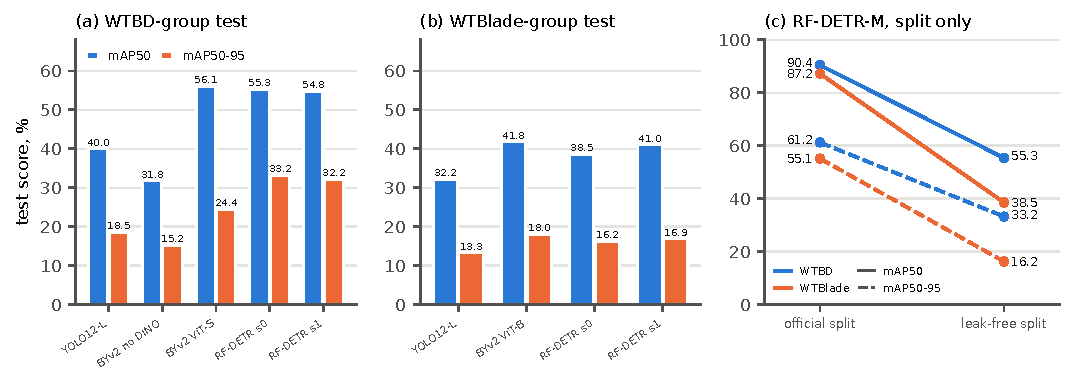
\includegraphics[width=\textwidth]{fig17_benchmark}
\caption{(a, b) Leak-free test scores by model (BYv2: BladeYOLO-v2; s0, s1: seeds). (c) RF-DETR-M on the official and leak-free splits of the same data.}
\label{fig:benchmark}
\end{figure*}

\begin{figure*}[!t]
\centering
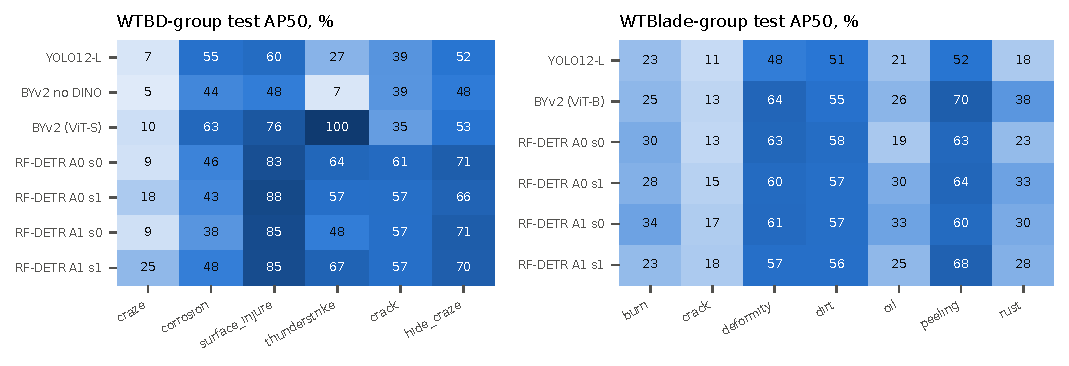
\includegraphics[width=0.96\textwidth]{fig24_per_class}
\caption{Per-class test \apfifty on the leak-free benchmarks. Note the seed-to-seed swings within RF-DETR on rare classes (craze 9--25, thunderstrike 48--67), and BladeYOLO-v2's thunderstrike 100, which rests on 3 test scenes.}
\label{fig:perclass}
\end{figure*}

Four points stand out:
\begin{itemize}
\item \textbf{The ranking depends on the dataset.} RF-DETR-M leads on WTBD-group by 7--9 \mcoco points over BladeYOLO-v2. On WTBlade-group, however, the frozen ViT-B BladeYOLO-v2 (18.0) is ahead of every RF-DETR run, RF-DETR-FP included (16.1--17.3). A ``generic detector is strongest'' claim holds on one benchmark.
\item \textbf{On WTBD the RF-DETR gain is box quality, not finding.} RF-DETR-M's \mfifty is level with BladeYOLO-v2 (55.3 and 53.2 against 56.1), while its \mcoco is 7--9 points higher. This matches the extent analysis of Section~\ref{sec:anatomy}.
\item \textbf{Classification costs RF-DETR points.} Scoring A0 with classes merged gives 66.1/40.5 on WTBD-group and 50.1/21.3 on WTBlade-group (Table~\ref{tab:g28}), about 11 \apfifty points above its class-aware score. BladeYOLO-v2's class-agnostic and class-aware \apfifty are about equal (56.3 against 56.1), while YOLO12-L shows a gap like RF-DETR's (48.5 against 40.0).
\item \textbf{The earlier BladeYOLO-v2 win over YOLO12-L rests largely on thunderstrike.} The scene bootstrap gives $+16.1$ \ci{+2.5}{+28.4} \mfifty and $+5.9$ \ci{+0.5}{+16.9} \mcoco. Without the two classes seen in at most 3 test scenes, however, the \mfifty gain is $+5.2$ \ci{-2.7}{+13.5}.
\end{itemize}

\subsection{RF-DETR-FP: Pre-Registered Test}
\label{sec:fp-results}
\textbf{Protocol} (G29, fixed before any run). Each RF-DETR-FP run is paired with an existing run of identical recipe on the same hardware type (Kaggle T4, fp16). The primary claim P compares FP and A0 on leak-free test \mcoco with the paired scene bootstrap of~\eqref{eq:bootstrap}, averaged over seeds 0 and 1 (2{,}000 replicates). It passes if the point estimate is $>0$ on each dataset and the dataset mean has $P(>0)\geq0.95$; this is the bar G27 failed. Reported with it, and not gating, are the validation split in the same form, WTBD-group without its six pixel-twin test images, per-class AP, the error anatomy and a comparison with every other architecture. Two mechanism predictions were also written down: that the gain is larger on WTBlade-group than on WTBD-group, and that on WTBD it sits in the rare, confusable classes. A secondary claim S asks the same question at 25\% labels (FP against V1 over four subsets). The official protocols are benchmark entries, not tests (Section~\ref{sec:official}).

\begin{table}[!t]
\centering
\caption{G29 primary claim (P): RF-DETR-FP $-$ RF-DETR-M (A0), leak-free \mcoco, paired scene bootstrap, mean of seeds 0 and 1.}
\label{tab:g29}
\footnotesize
\setlength{\tabcolsep}{2.2pt}
\begin{tabular}{@{}l l l l l@{}}
\toprule
& A0 s0 / s1 & FP s0 / s1 & FP $-$ A0 [95\% CI] & $P(>0)$ \\
\midrule
WTBD-group test & 33.2 / 31.2 & 34.3 / 34.5 & $+2.18$ \ci{-0.8}{+4.4} & 0.916 \\
WTBlade-group test & 16.2 / 16.9 & 17.3 / 17.2 & $+0.72$ \ci{-0.6}{+1.9} & 0.866 \\
\textbf{mean, test} & & & $\mathbf{+1.45}$ \ci{-0.2}{+2.7} & \textbf{0.958} \\
\midrule
WTBD-group val & 40.1 / 40.2 & 42.2 / 39.0 & $+0.43$ \ci{-3.1}{+3.3} & 0.569 \\
WTBlade-group val & 15.7 / 16.6 & 16.1 / 16.1 & $-0.02$ \ci{-2.8}{+2.2} & 0.465 \\
mean, val & & & $+0.20$ \ci{-2.0}{+1.9} & 0.526 \\
\bottomrule
\end{tabular}
\end{table}

\begin{figure*}[!t]
\centering
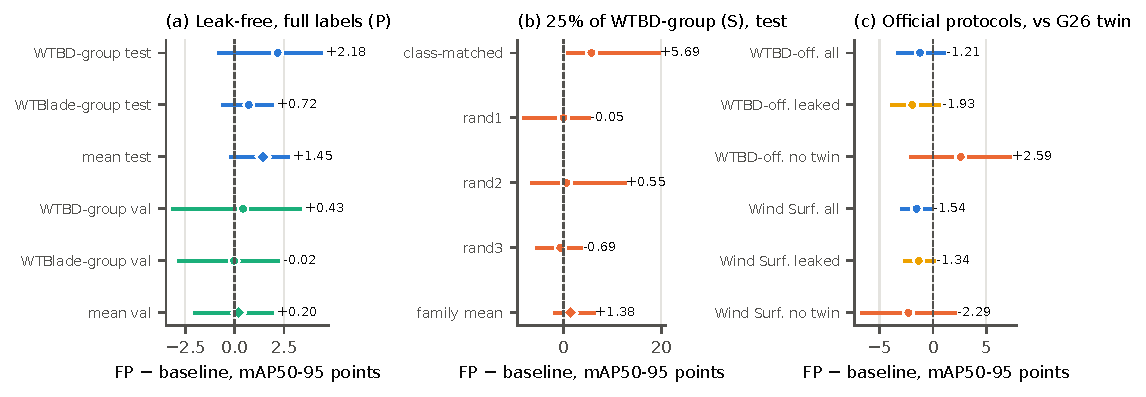
\includegraphics[width=\textwidth]{fig29_g29_effects}
\caption{RF-DETR-FP paired effects in \mcoco points with 95\% intervals. (a) Primary claim on the leak-free benchmarks, test (blue) and validation (green); diamonds mark dataset means. (b) Secondary claim at 25\% of WTBD-group scenes, four subsets, test. (c) Official protocols against the G26 twin, on all, leaked and no-twin test images (image bootstrap).}
\label{fig:g29-effects}
\end{figure*}

\textbf{Result.} By the pre-registered rule the primary claim \emph{passes} (Table~\ref{tab:g29}, Fig.~\ref{fig:g29-effects}a). The effect is positive on both datasets, and the mean has $P(>0)=0.958$ against a bar of 0.95. On test, both FP seeds are above both A0 seeds on both datasets. RF-DETR-FP reaches 34.4 \mcoco on WTBD-group (mean of seeds), the best result on that benchmark by any model, and 17.3 on WTBlade-group. \mfifty rises more than \mcoco: 54.3 to 58.9 on WTBD-group and 40.0 to 41.0 on WTBlade-group. Without WTBD-group's six pixel-twin test images the gain is $+1.97$ (31.7 to 33.6), so those images do not carry it.

\textbf{Honest strength: narrow.} Validation does not confirm the gain ($+0.20$, $P=0.53$). The rule is decided on test, as for G27, so this does not change the verdict. It is, however, the pattern of an earlier hypothesis (H5) that passed narrowly on test with a flat validation result and then failed to replicate. The WTBD effect ($+2.2$) is about the size of A0's own seed spread there (33.2 against 31.2). And both mechanism predictions fail. The gain is larger on WTBD-group than on WTBlade-group ($+2.18$ against $+0.72$), the reverse of the prediction. On WTBD it sits in surface\_injure ($+5.8$) and craze ($+3.8$) rather than in thunderstrike ($+1.1$) and crack ($+1.4$) (Fig.~\ref{fig:g29-perclass}). The error anatomy barely moves: hits rise from 71.1 to 71.9\% and ``ranked low'' falls from 25.1 to 24.3\% on WTBD, and ``no box'' falls from 7.2 to 6.5\% on WTBlade. The effect looks real on test, but it is not where the evidence that motivated it said it would be.

\textbf{Against other architectures.} On WTBD-group, RF-DETR-FP (34.4) is above every other architecture: BladeYOLO-v2 24.4, YOLO12-L 18.5 and RF-DETR-M 31.2--33.2. On WTBlade-group (17.3) it is still below the frozen-DINOv3 BladeYOLO-v2 ViT-B (18.0, single run), though above YOLO12-L (13.3). The pre-registered ``beats every architecture on both leak-free tests'' condition is therefore \emph{not} met.

\begin{table}[!t]
\centering
\caption{G29 secondary claim (S): 25\% of WTBD-group scenes, RF-DETR-FP $-$ RF-DETR-M (V1), seed 0, 576\,px, \mcoco, scene bootstrap.}
\label{tab:g29s}
\footnotesize
\setlength{\tabcolsep}{3pt}
\begin{tabular}{@{}l l l l l@{}}
\toprule
Subset & V1 & FP & FP $-$ V1 [95\% CI] & $P(>0)$ \\
\midrule
class-matched & 18.9 & 24.6 & $+5.69$ \ci{+0.8}{+19.5} & 0.981 \\
random 1 & 20.5 & 20.4 & $-0.05$ \ci{-8.1}{+5.2} & 0.420 \\
random 2 & 21.5 & 22.1 & $+0.55$ \ci{-6.5}{+12.5} & 0.592 \\
random 3 & 14.7 & 14.1 & $-0.69$ \ci{-5.5}{+3.6} & 0.413 \\
family mean, test & & & $+1.38$ \ci{-1.8}{+6.2} & 0.856 \\
family mean, val & & & $+1.41$ \ci{-0.3}{+4.2} & 0.953 \\
\bottomrule
\end{tabular}
\end{table}

\textbf{Low labels.} The secondary claim fails (Table~\ref{tab:g29s}). The family mean is $+1.38$, $P=0.856$, positive on 2 of 4 subsets, although validation is positive on all four. At 25\% labels, RF-DETR-FP is therefore not the low-label lever that frozen DINOv3 was for the YOLO family. Subset luck still dominates: the class-matched subset alone moves by $+5.7$.

\begin{figure}[!t]
\centering
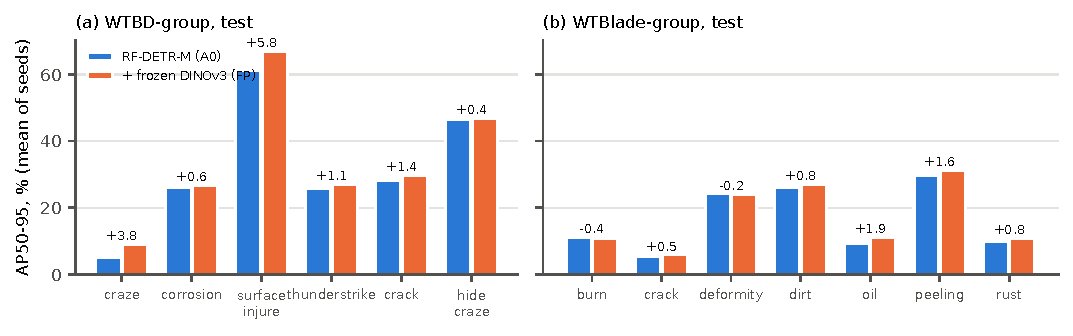
\includegraphics[width=\linewidth]{fig31_g29_perclass}
\caption{Per-class test AP$_{50:95}$ of RF-DETR-M (A0) and RF-DETR-FP, mean of two seeds; the label above each pair is the change. The gain sits in frequent classes (surface\_injure, craze; oil, peeling), not in the rare ones the motivating evidence pointed to.}
\label{fig:g29-perclass}
\end{figure}

\begin{figure*}[!t]
\centering
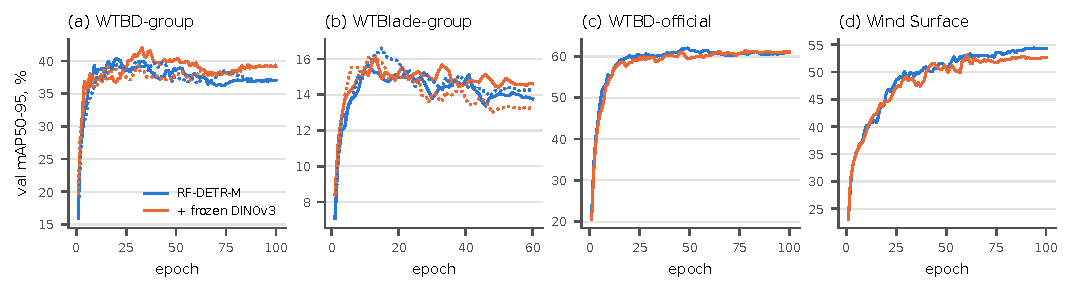
\includegraphics[width=\textwidth]{fig30_g29_curves}
\caption{Validation \mcoco (EMA) per epoch, RF-DETR-M against RF-DETR-FP with identical recipes. Solid: seed 0; dotted: seed 1. (a, b) Leak-free benchmarks. (c, d) Official protocols. On the leak-free splits both models peak early and drift, so EMA checkpoint selection matters. FP's curve stays higher late in training on WTBD-group, but its selected checkpoint does not separate on validation.}
\label{fig:g29-curves}
\end{figure*}

\begin{figure*}[!t]
\centering
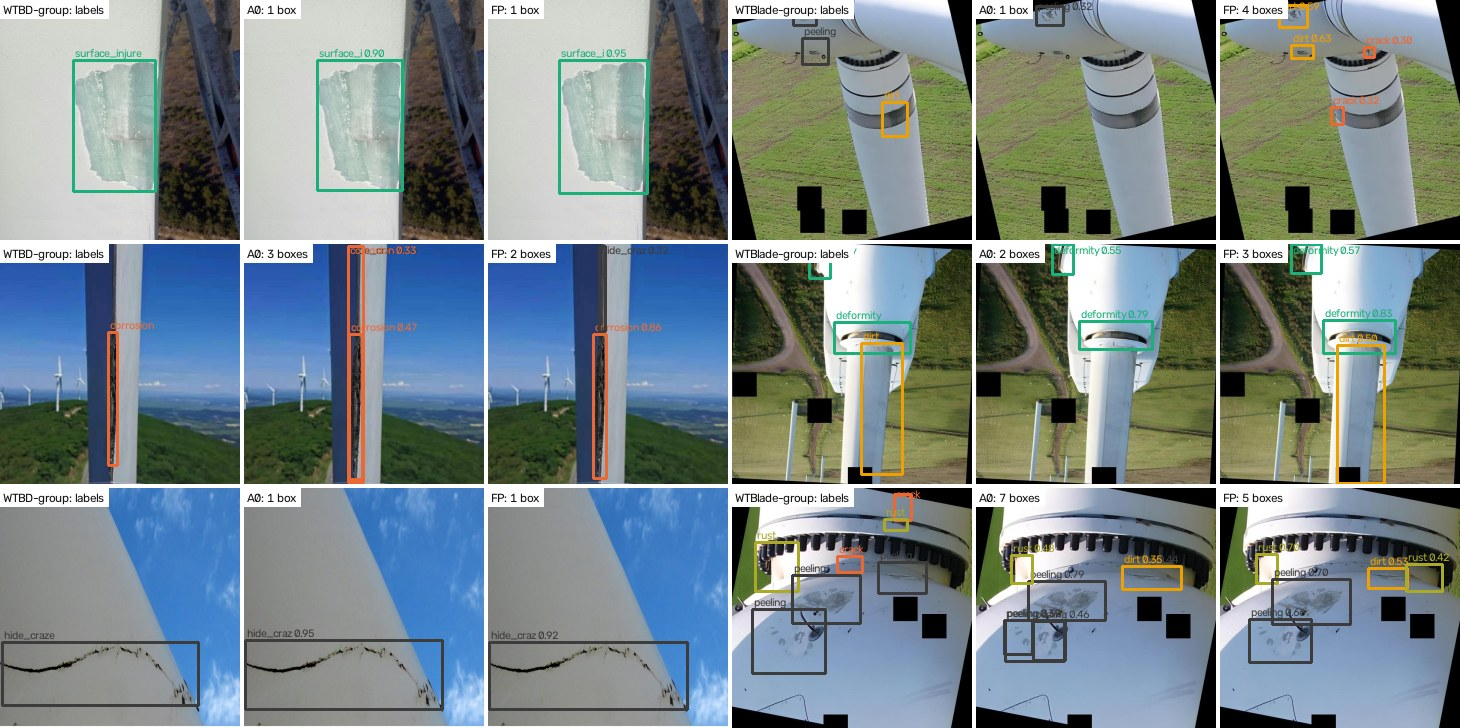
\includegraphics[width=\textwidth]{fig33_g29_predictions}
\caption{Labels, RF-DETR-M (A0) and RF-DETR-FP (seed 0) on random test images of WTBD-group (left three columns) and WTBlade-group (right three), fixed seed, boxes with confidence $\geq0.3$. Black squares in WTBlade-group are the Roboflow export's offline cutout, which the frames retain.}
\label{fig:g29-pred}
\end{figure*}

Fig.~\ref{fig:g29-curves} shows the training curves, and Fig.~\ref{fig:g29-pred} shows predictions on random test images. On the official protocols (Table~\ref{tab:tuning}, Fig.~\ref{fig:g29-effects}c), RF-DETR-FP raises \mfifty and lowers \mcoco. Its WTBD change sits on the no-twin images, and on Wind Surface it does not close the gap to BladeYOLO ($-4.4$ \mfifty, $-5.7$ \mcoco). By class on Wind Surface, thunderstrike improves (\apfifty 69 to 76) and surface\_eye falls (93 to 88).

\textbf{Verdict.} RF-DETR-FP passes its pre-registered primary test, by a narrow margin that validation does not support. It is the strongest leak-free RF-DETR result in this study, and the best WTBD-group result of any model. The honest wording is: a small gain ($+1.5$ points mean) that passes on test and is not confirmed on validation. It is not a low-label method, its gain is not where the motivating evidence predicted, and on the leaky official protocols it does not beat BladeYOLO's Wind Surface numbers. As pre-registered, we ran no rescue runs.

\subsection{Where the YOLO-Family Advantage Comes From: DINOv3 Ablation}
\label{sec:ablation}
We removed only the frozen DINOv3 features from BladeYOLO-v2, keeping deformable refinement, selective scan and WIoU. We then trained at 25\%, 50\% and 100\% of the labelled scenes (Table~\ref{tab:ablation}, Fig.~\ref{fig:curve}).

\begin{table*}[!t]
\centering
\caption{DINOv3 ablation and learning curve on WTBD-group: test \mcoco by labelled fraction, scene bootstrap for differences. \hlnote{} (among the three models)}
\label{tab:ablation}
\footnotesize
\begin{tabular}{@{}l l l l@{}}
\toprule
& 25\% of scenes & 50\% & 100\% \\
\midrule
BladeYOLO-v2 (frozen DINOv3 ViT-S) & \best{7.6} (3 seeds) & \best{17.5} & \best{24.2} (2 seeds) \\
BladeYOLO-v2 without DINOv3 & 3.7 (2 seeds) & 8.8 & 15.2 \\
YOLO12-L (stock) & \second{4.1} & \second{9.9} & \second{18.5} \\
\midrule
DINOv3 gain & $+3.9$ \ci{+2.5}{+10.1} & $+8.8$ \ci{+4.0}{+22.1} & $+9.0$ \ci{+4.0}{+20.5} \\
DINOv3 gain, 4 well-represented classes & $+4.4$ \ci{+2.3}{+11.1} & $+6.1$ \ci{+2.2}{+17.9} & $+4.9$ \ci{-1.8}{+10.3} \\
YOLO12-L $-$ BladeYOLO-v2 without DINOv3 & $+0.4$ & $+1.1$ & $+3.3$ \ci{-0.2}{+13.1} \\
\bottomrule
\end{tabular}
\end{table*}

\begin{figure}[!t]
\centering
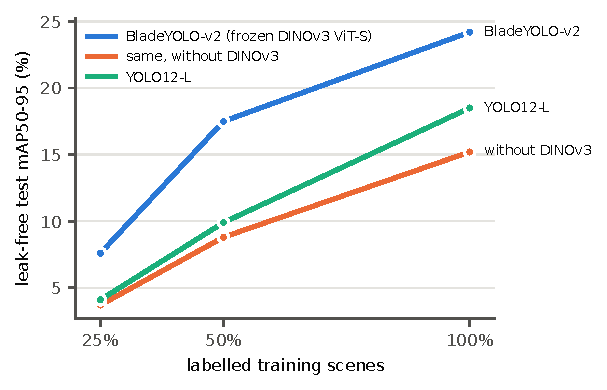
\includegraphics[width=0.92\linewidth]{fig4_dinov3_learning_curve}
\caption{Learning curves with and without frozen DINOv3 on WTBD-group. The modules around DINOv3 do not put the model above stock YOLO12-L.}
\label{fig:curve}
\end{figure}

Without DINOv3, BladeYOLO-v2 equals or trails stock YOLO12-L at every data size. The advantage is therefore the features, not the architecture around them. We first read it as a low-data advantage; the 50\% and 100\% runs corrected that, since the absolute gain does not shrink with data. Only the relative gain does, from $2.0\times$ to $1.6\times$. Labelled scenes still pay throughout: the learning curve has not flattened at 100\%. This claim concerns our components. BladeYOLO's exact style-injection, WTConv and Cross-Mamba modules were reimplemented only before our code audit, so we make no claim about them.

\textbf{Backbone size at 25\%} (Table~\ref{tab:backbone}). A larger frozen backbone helps up to ViT-B, and ViT-L adds nothing further. This is why RF-DETR-FP uses ViT-B.

\begin{table}[!t]
\centering
\caption{Frozen DINOv3 size at 25\% of WTBD-group scenes: test scores by Ultralytics \texttt{val}, per seed and mean; differences by scene bootstrap, \mcoco points. \hlnote{}}
\label{tab:backbone}
\scriptsize
\setlength{\tabcolsep}{1.8pt}
\begin{tabularx}{\linewidth}{@{}l X c c l@{}}
\toprule
Backbone & Per seed (50/50:95) & Mean 50 & Mean 50:95 & $\Delta$\mcoco [95\% CI] \\
\midrule
none (2) & 11.4/4.4, 8.1/3.1 & 9.8 & 3.8 & none$-$S: $-3.9$ \ci{-10.1}{-2.5} \\
ViT-S/16 (3) & 23.2/8.2, 22.4/8.7, 18.4/6.8 & 21.3 & 7.9 & \\
ViT-B/16 (2) & 25.2/10.2, 28.3/11.6 & \second{26.8} & \second{10.9} & B$-$S: $+2.8$ \ci{+0.4}{+9.6} \\
ViT-L/16 (2) & 33.7/11.5, 30.1/10.9 & \best{31.9} & \best{11.2} & L$-$B: $+0.3$ \ci{-4.0}{+3.1} \\
\bottomrule
\end{tabularx}
\end{table}

\textbf{Fine-tuned against frozen foundation features, 25\% labels, same subsets (V1).} RF-DETR-M beats BladeYOLO-v2 ViT-B by $+7.3$ \ci{+2.3}{+11.9} \mcoco (seed 0) and $+8.3$ \ci{+4.5}{+15.0} (seed 1), and it is positive on 4 of 4 subsets at each seed. As a controlled comparison, freezing RF-DETR's own encoder lowers test \mcoco from 18.9 to 12.3 on WTBD and from 13.2 to 8.7 on WTBlade. Input resolution (G24) adds $+1.0$ from 576 to 768\,px on WTBD ($P=0.958$) and $-0.1$ on WTBlade, whose frames are natively 640\,px.

\subsection{Training Behaviour}
Fig.~\ref{fig:training} shows validation curves from the final-phase runs. RF-DETR peaks early and then drifts down, which is why EMA checkpoint selection matters. In contrast, YOLO12-L on WTBlade-group rises almost linearly until about epoch 43 of 50, so its row may understate it. Fig.~\ref{fig:examples} shows training and validation batches, and Fig.~\ref{fig:diagnostics} confusion matrices and a PR curve. In the matrices, columns are true classes. The bottom row shows missed labels (crack 18\% on WTBD-group and 27\% on WTBlade-group for YOLO12-L), and the right column shows where false positives go. The strongest confusions involve rare classes: YOLO12-L calls 54\% of thunderstrike labels craze on WTBD-group test.

\begin{figure*}[!t]
\centering
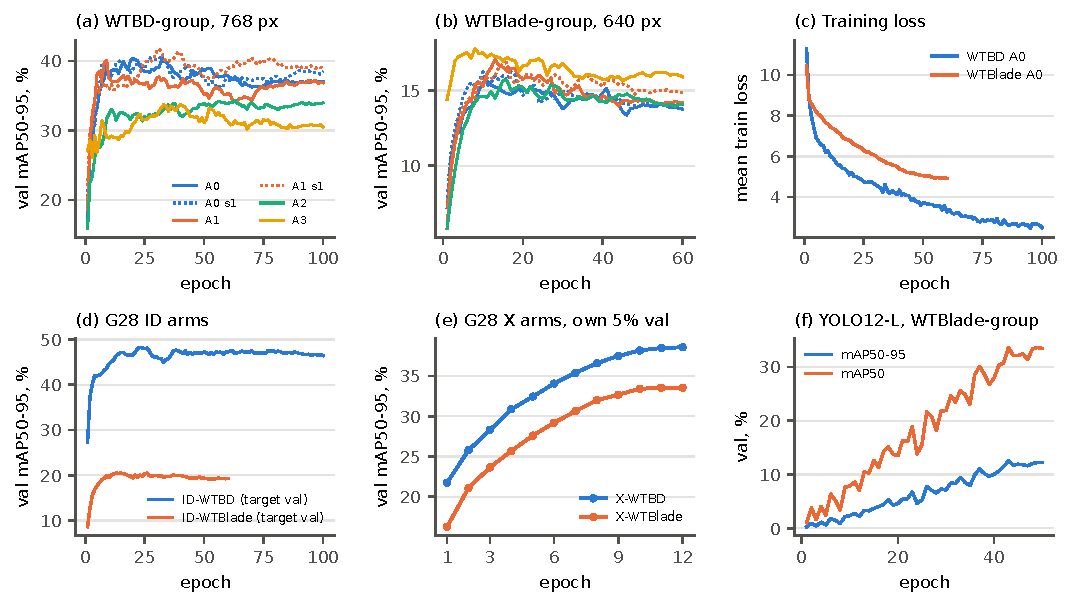
\includegraphics[width=\textwidth]{fig15_training_curves}
\caption{Training records. (a, b) Validation \mcoco of the G27 arms; dotted lines are seed 1. (c) Training loss of A0. (d) G28 ID arms on target validation. (e) G28 X arms on their own held-out 5\%, not comparable with (d) since the images differ. (f) YOLO12-L on WTBlade-group.}
\label{fig:training}
\end{figure*}

\begin{figure*}[!t]
\centering
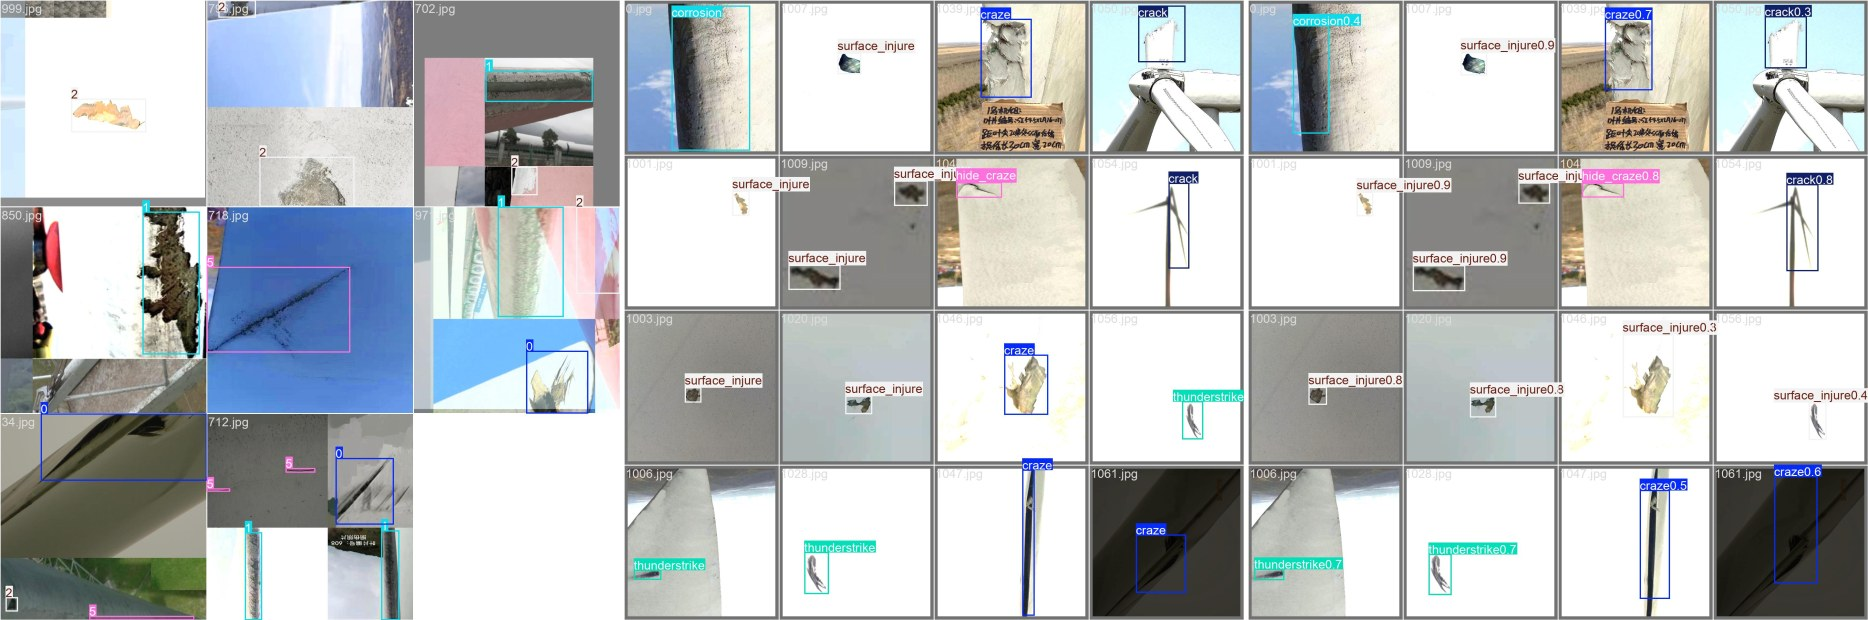
\includegraphics[width=\textwidth]{fig26_training_examples}
\caption{BladeYOLO-v2 on WTBD-group, from the training run. Left: a training batch after mosaic and flips. Middle: a validation batch with its labels. Right: the same batch with predictions.}
\label{fig:examples}
\end{figure*}

\begin{figure}[!t]
\centering
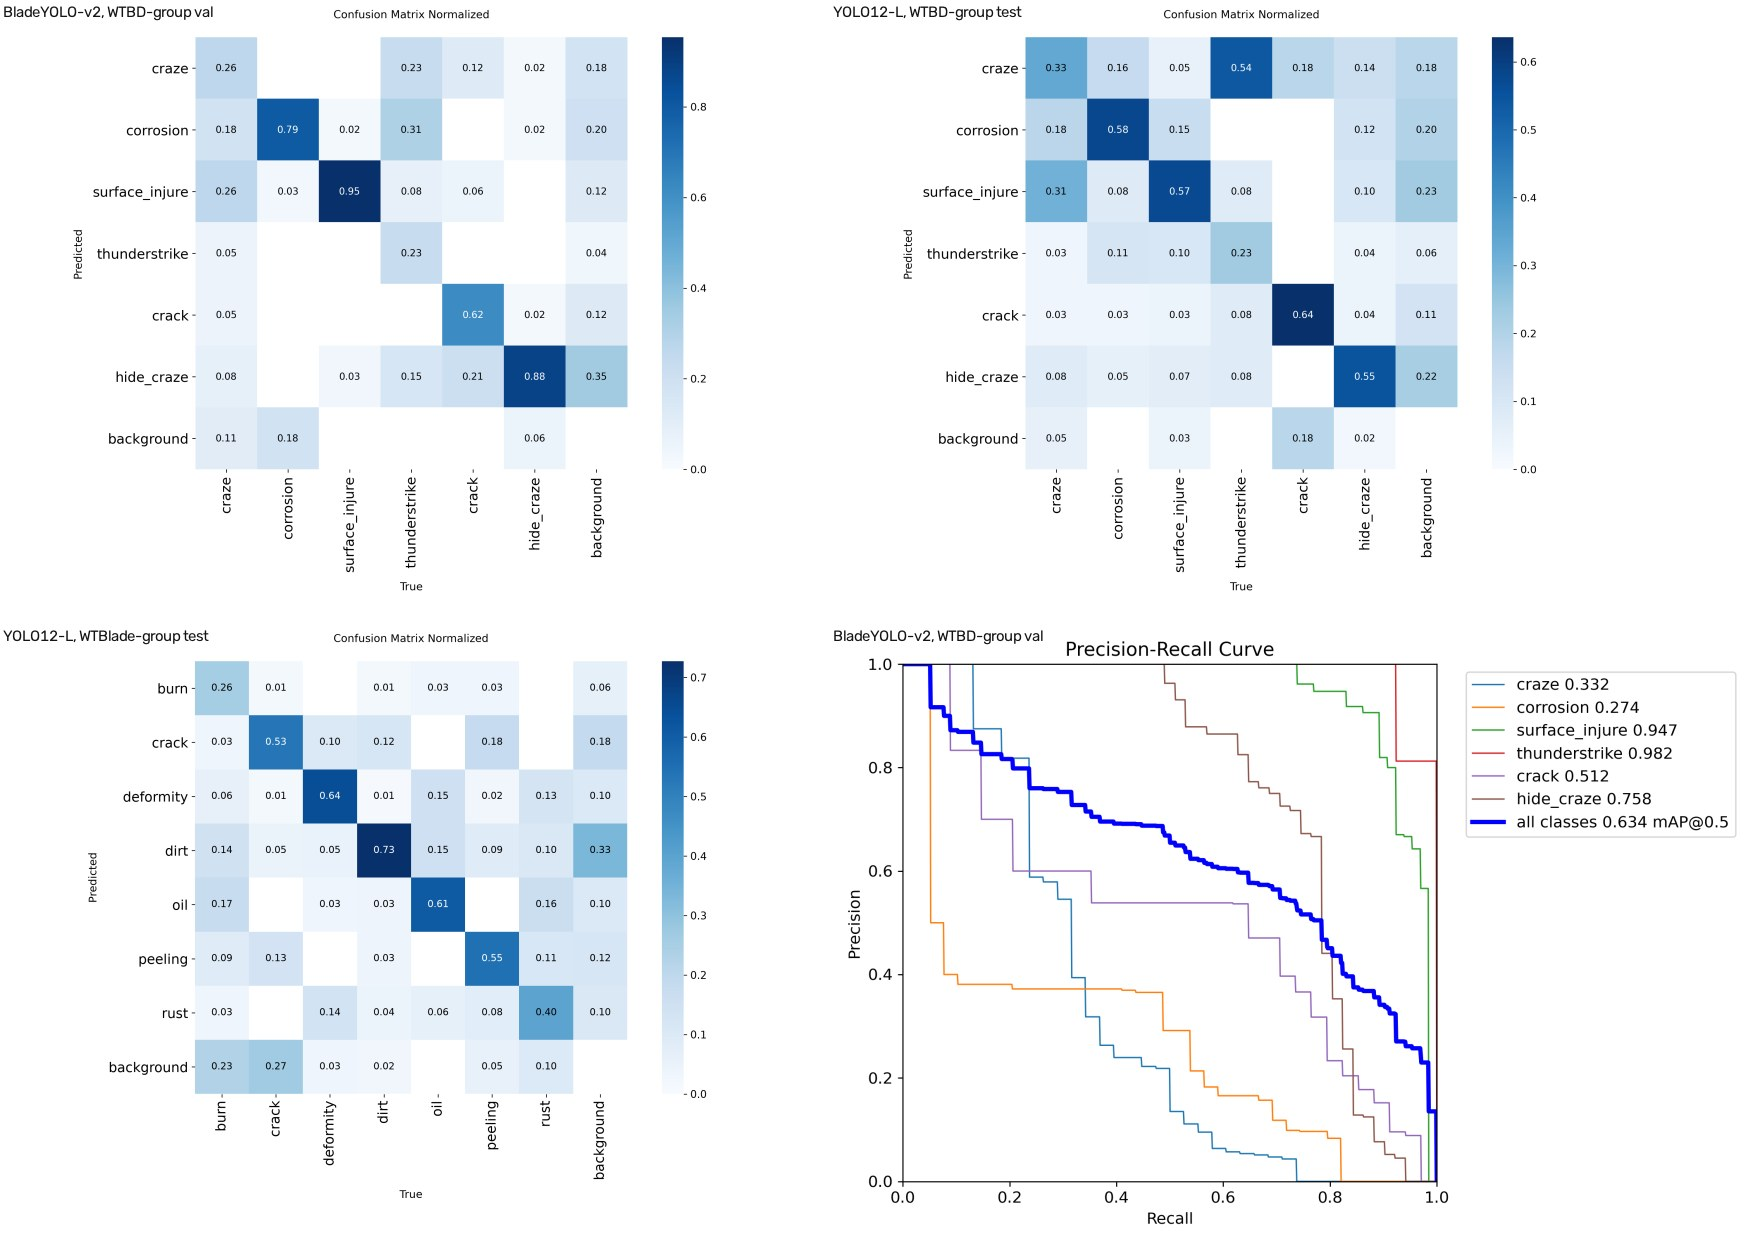
\includegraphics[width=\linewidth]{fig27_diagnostics}
\caption{Diagnostics. Normalised confusion matrices: BladeYOLO-v2 on WTBD-group validation, YOLO12-L on WTBD-group test and YOLO12-L on WTBlade-group test. Bottom right: PR curves by class of BladeYOLO-v2 on WTBD-group validation.}
\label{fig:diagnostics}
\end{figure}
